 \chapter{Methodology}\label{ch:methodology}

\section{Introduction}\label{sec:intro}

This chapter describes the development approach for \textbf{Collective}, a mobile journaling application. The methodology covers framework selection, AI implementation, and cloud service integration.

Collective addresses a specific problem: traditional journaling provides focus but lacks digital features like search and organization, while existing digital journaling apps overwhelm users with complex interfaces. The solution maintains journaling simplicity while adding intelligent features behind the scenes.

The development approach prioritizes user experience through rapid iteration and continuous feedback. Key challenges include cross-platform compatibility, offline functionality, data synchronization, and privacy protection. Rapid Application Development (RAD) methodology was chosen to handle these requirements effectively.

\section{Rapid Application Development (RAD) Methodology}\label{sec:rad}

RAD methodology was selected for developing Collective because it emphasizes quick prototyping and user feedback integration. This approach suits mobile applications where user experience is critical and requirements may change based on testing.

RAD consists of four phases: Requirements Planning, User Design, Construction, and Cutover. The methodology allows parallel development of different components, which is essential when integrating AI processing with user interface design.

\begin{figure}[H]
\centering
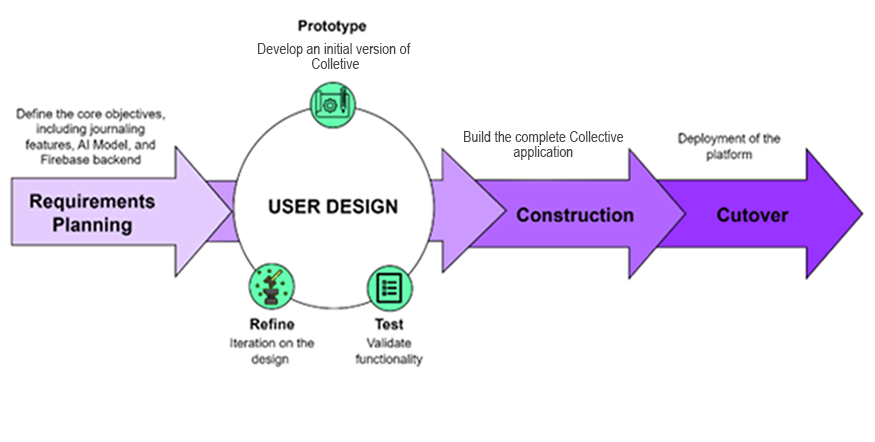
\includegraphics[width=0.8\textwidth]{files/imgs/RAD.png}
\caption{Rapid Application Development (RAD) Methodology Phases}
\label{fig:rad-methodology}
\end{figure}

RAD was chosen for several reasons:

\textbf{User Focus:} The methodology emphasizes user involvement, which aligns with creating an intuitive journaling experience that maintains simplicity while incorporating AI capabilities.

\textbf{Quick Prototyping:} Rapid prototyping enables testing different approaches to AI integration and user interface design. This is crucial for a journaling app where user experience directly impacts adoption.

\textbf{AI Integration Flexibility:} RAD accommodates the experimental nature of AI development, allowing refinement of natural language processing and mood detection based on real-world testing.

\textbf{Cross-Platform Support:} The methodology supports parallel development for consistent experiences across iOS and Android using Flutter framework.

The RAD phases for Collective:

\textbf{Requirements Planning:} Analysis of user journaling behaviors, identification of pain points in existing solutions, and specification of AI capabilities needed without adding complexity.

\textbf{User Design:} Creation of wireframes and prototypes that maintain simplicity while accommodating AI features. Includes user testing to validate the swipe-to-save interaction.

\textbf{Construction:} Implementation using Flutter framework, Firebase integration for authentication and storage, AI processing development, and offline functionality creation.

\textbf{Cutover:} Deployment preparation, cross-platform testing, performance optimization, and monitoring system establishment.

\section{Requirement planning}\label{sec:requirementPlanning}   
\subsection{Software Requirements}\label{subsec:softwareRequirements}
\subsection{Hardware Requirements}\label{subsec:hardwareRequirements}
\subsection{Use Case Diagram}\label{subsec:usecaseDiagram}
\subsection{Use Case Description}\label{subsec:usecaseDescription}

\section{User design}\label{sec:userDesign}